%; whizzy chapter
% -initex iniptex -latex platex -format platex -bibtex jbibtex -fmt fmt
% 以上 whizzytex を使用する場合の設定。

%     Kansai Debian Meeting resources
%     Copyright (C) 2007 Takaya Yamashita
%     Thank you for Tokyo Debian Meeting resources

%     This program is free software; you can redistribute it and/or modify
%     it under the terms of the GNU General Public License as published by
%     the Free Software Foundation; either version 2 of the License, or
%     (at your option) any later version.

%     This program is distributed in the hope that it will be useful,
%     but WITHOUT ANY WARRANTY; without even the implied warranty of
%     MERCHANTABILITY or FITNESS FOR A PARTICULAR PURPOSE.  See the
%     GNU General Public License for more details.

%     You should have received a copy of the GNU General Public License
%     along with this program; if not, write to the Free Software
%     Foundation, Inc., 51 Franklin St, Fifth Floor, Boston, MA  02110-1301 USA

%  preview (shell-command (concat "evince " (replace-regexp-in-string "tex$" "pdf"(buffer-file-name)) "&"))
% 画像ファイルを処理するためにはebbを利用してboundingboxを作成。
%(shell-command "cd image200708; ebb *.png")

%%ここからヘッダ開始。

\documentclass[mingoth,a4paper]{jsarticle}
\usepackage{kansaimonthlyreport}
\usepackage[dvips]{xy}


% 日付を定義する、毎月変わります。
\newcommand{\debmtgyear}{2012}
\newcommand{\debmtgdate}{25}
\newcommand{\debmtgmonth}{3}
\newcommand{\debmtgnumber}{57}

\begin{document}

\begin{titlepage}

% 毎月変更する部分、本文の末尾も修正することをわすれずに

 第\debmtgnumber{}回 関西 Debian 勉強会資料

\vspace{2cm}

\begin{center}
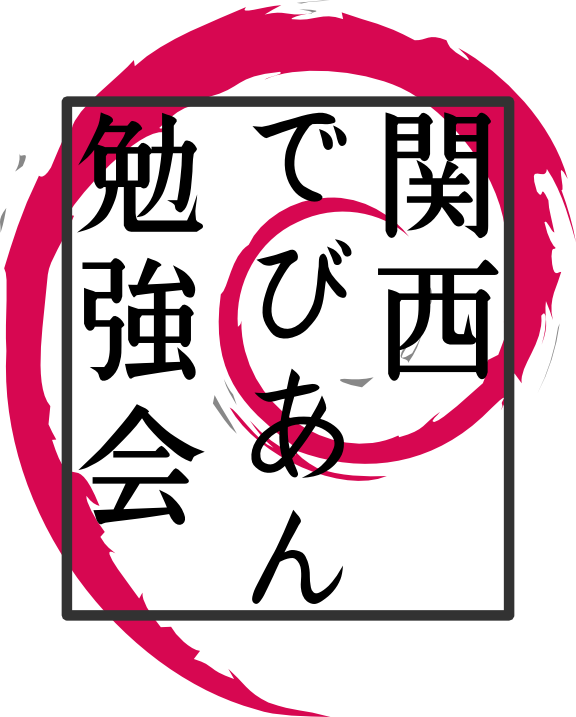
\includegraphics{image200802/kansaidebianlogo.png}
\end{center}

\begin{flushright}
\hfill{}関西 Debian 勉強会担当者 佐々木・倉敷・のがた・かわだ \\
\hfill{}\debmtgyear{}年\debmtgmonth{}月\debmtgdate{}日
\end{flushright}

\thispagestyle{empty}
\end{titlepage}

\dancersection{Introduction}{Debian JP}

 関西Debian勉強会はDebian GNU/Linuxのさまざまなトピック
 (新しいパッケージ、Debian特有の機能の仕組、Debian界隈で起こった出来事、
 などなど)について話し合う会です。

 目的として次の三つを考えています。
 \begin{itemize}
  \item MLや掲示板ではなく、直接顔を合わせる事での情報交換の促進
  \item 定期的に集まれる場所
  \item 資料の作成
 \end{itemize}

 それでは、楽しい一時をお楽しみ下さい。

\newpage

\begin{minipage}[b]{0.2\hsize}
 {\rotatebox{90}{\fontsize{80}{80}
{\gt 関西 Debian 勉強会}}}
\end{minipage}
\begin{minipage}[b]{0.8\hsize}
\hrule
\vspace{2mm}
\hrule
\setcounter{tocdepth}{1}
\tableofcontents
\vspace{2mm}
\hrule
\end{minipage}

\dancersection{最近のDebian関係のイベント報告}{Debian JP}

\subsection{第 56 回関西 Debian 勉強会}
56 回目の関西 Debian 勉強会は 2月 26 日に
福島区民センターで開催されました。

月刊 t-code パッケージ修正「emacs24で問題なく使えるt-code.debを作った話」、
月刊 Debian Policy、そして「Autofs と pam\_chroot で作るマルチユーザ環境」という発表がありました。
残念なら佐々木は職場のでの同時多発ストレージテロに遭遇してしまい、
ちゃんとお話を伺えなかったのですが非常に熱い議論が行なわれいた模様です。

\subsection{第 86 回東京エリア Debian 勉強会}
86 回目の東京エリア Debian 勉強会が 3 月 17 日に
OSC Tokyo Spring において開催されました。\\
「Apache2/ HTTP サーバから始めるDebian」と題して、
Webサーバとして世界で一番採用されているLinuxディストリビューションである Debian の Apache2 について、「ユーザ視点の勉強会」が行なわた模様です。
また GPG キーサインパーティも開催されました。

\clearpage

\dancersection{事前課題}{Debian JP}

今回は以下の課題を出題しました.
\begin{screen}
  \begin{enumerate}
  \item Debian Policy の第5章を読んできて下さい。
  \item 何か一つパッケージを取得して
    debian/control ファイルを読んできてください。
    そのパッケージの control ファイルの内容について簡単に、
    わからない箇所は調べて、当日紹介して下さい。
  \item 勉強会開催をどのような媒体、方法で告知を出してもらいたいですか。
  \end{enumerate}
\end{screen}

参加者の皆さんの解答は以下の通りです.

\begin{prework}{ 水野源 }
  (無回答)
\end{prework}

\begin{prework}{ 榎真治 }
  (無回答)
\end{prework}

\begin{prework}{ 山下康成 }
  げほげほっ!
\end{prework}

\begin{prework}{ 川江 }
  \begin{enumerate}
  \item 読んできます
  \item 努力します
  \item 今のままでいいと思いますが、個人的な事情として「多忙」な人が気軽
    に『参加』できるような「方法」があればありがたいです。
  \end{enumerate}
\end{prework}

\begin{prework}{ かわだてつたろう }
  \begin{enumerate}
  \item 読んでおきます。
  \item cpp の control を読みました。
    \begin{itemize}
    \item sid:amd64 で "Multi-Arch: allowd" となっているのはこのパッケージだけのようです。どのような場合に指定するとよいのか今一つわかっていません。
    \end{itemize}
  \item Debian JP のサイト。。。
  \end{enumerate}
\end{prework}

\begin{prework}{ kozo2 }
  \begin{enumerate}
  \item 読みます
  \item t-codeの読みます
  \item 媒体,方法 twitter, ML 位しか思い浮かばんとです
  \end{enumerate}
\end{prework}

\begin{prework}{ 山田 洋平 }
  \begin{enumerate}
  \item 当日までに読んで来ます。
  \item 当日までに読んで来ます。
  \item カレンダーのイベント
  \end{enumerate}
\end{prework}

\begin{prework}{ 酒井 忠紀 }
  \begin{enumerate}
  \item ざっくり読みました
  \item ruby1.8 の debian/controlファイルをざっくり読みました。
    今回、発表させて頂く Konoha に関連することですが、
    debian/controlファイルに関する疑問点を以下に記述します。
    \begin{description}
    \item[Maintainer]
      emailアドレスの名前にピリオドが含まれていると問題が
      あるようですが、以下以外であれば、問題ない認識で
      よいでしょうか?
      \begin{itemize}
      \item 連続してピリオドを使用している
      \item '@' の直前にピリオドを使用している
      \end{itemize}
    \item[Priority]
      新規パッケージで他と競合しないものは、optional で
      よい認識で問題ないでしょうか?
    \item[Architecture]
      ここで指定するアーキテクチャが、実際に自動ビルドされて
      Debianアーカイブに置かれるアーキテクチャになる認識でよいで
      しょうか?
    \end{description}
  \item 現状のままでもよいと思いますが、ATNDなどを使用すると、より多くの人の目に留まるかもしれません。
  \end{enumerate}
\end{prework}

\begin{prework}{ 山城の国の住人 久保博 }
  \begin{itemize}
  \item はい、読みます
  \item 当日までに何とか。
  \item 発表に関係の深い単語のハッシュタグをつけて twitter で
  \end{itemize}
\end{prework}

\begin{prework}{ よしだともひろ }
  \begin{itemize}
  \item Debian JP Projectの日本語訳に一通り目を通しました。
  \item e2wmのdebian/controlを見ました
  \item Debian JPのメーリングリストでよいと思います。
  \end{itemize}
\end{prework}

\begin{prework}{ のがたじゅん }
  OSC愛媛から日曜の朝、鈍行で帰るのでたどり着けませーん。
  \begin{itemize}
  \item 前はmixiにも告知を流してたけど、今ならぐぐたすかfacebookか…といっても、あまりフィットする感じではないのでtwitterぐらいなのかなぁと思ったり。
  \end{itemize}
\end{prework}

\begin{prework}{ yyatsuo }
  3. 今のままで特に不都合無いです
\end{prework}

\begin{prework}{ 佐々木洋平 }
  \begin{itemize}
  \item 了解しました。
  \item {\tt{git.debian.org:/git/pkg-ruby-extras/pkg-ruby-extras.git}}
    以下にある control はひととおり目を通しています。
  \item twitter の通知の自動化はともかくとして、他になにか無いかなぁ.
    (人力ではなくて、適当に自動化できることが前提だけれど). 告知と、締切前の再告知とかできると良いのだけれど.
    新入生獲得(?)に繋がりそうな他のアイデアないかねぇ.
  \end{itemize}
\end{prework}

\clearpage

\dancersection{新年度からのネタ/スケジュールに関して}{司会: 佐々木洋平}

\subsection{はじめに}

常連さんもいらっしゃって定期的に10人強の参加が見込まれる本勉強会ですが、
毎度勉強会のネタをどうするのか、というのはなかなか決まりません。\footnote{%
  「呑み会で決まるのが関西Debianクオリティ」なのかもしれませんが(笑)}。参
加者持ち寄りで楽しい話が伺えたりするのは大変嬉しいのですが、
(結果として)毎年必ずやっているようなお題は、
年度頭にスケジュールを決めてしまって定期的にやっても良いのじゃないのかな、
と思ったりもします。当然ながら中身を更新しつつですが%
\footnote{%
  debhelper を使った話から CDBS や dh の話になったり,
  source format が 1.0 から 3.0 になったり, 毎年変更点はあるものです}。

あとは新規参加者の確保、というのも一つの目標だったりします。
これを行なうにも、多少月毎のテーマが決まっていた方が参加しやすかったりしませんかね。

昨年12月の勉強会で「来年どんな話を聞きたいですか(したいですか)」というお話で、
参加者にいろいろお話を伺いました。
%
そこで上がっていた話題を列挙してみましょう(順番に特に意味はありません)。

\vspace{1.5em}
\begin{minipage}{.45\textwidth}
  \begin{itemize}
  \item DebianにおけるARM Cortexとのいろいろ
  \item パッケージ作成, debパッケージの作り方
  \item Blender関連
  \item BTSの歩き方
  \item WindowsユーザのためのDebian入門
  \item Debianデスクトップ入門
  \item Debianインストールハンズオン
  \end{itemize}
\end{minipage}
\begin{minipage}{.45\textwidth}
  \begin{itemize}
  \item LibreOffice入門
  \item KVM
  \item 組み込みDebian
  \item ライセンス
  \item live-build 3.x
  \item 月刊Debian Policy
  \item debian-el, debian.vim?
  \end{itemize}
\end{minipage}
\vspace{1.5em}

ついでに告知に関して。
現在は (1) ML での告知、(2) Web での告知、(3) Twitter \@debianjp での
告知が行なわれていますが (2) と (3) に関しては(困ったことに)結構忘れがちです。
これも今後どの様に行なうか考えてみたいです。

これらを踏まえて、ちょっと議論してみませんか?
皆さんの御知恵を拝借させて下さい。

\clearpage

\dancersection{Konoha の Debianパッケージ化について}{酒井 忠紀}
\subsection{はじめに}
Konoha を Debian パッケージにして sid にコミットしたいと考えています。
今回は、以下について説明します。
\begin{itemize}
\item Konoha の概要
\item パッケージ化の内容確認
\item スポンサーになってくださる方の相談
\end{itemize}

\subsection{Konoha の概要}

\subsubsection{Konoha とは}
Konoha は、静的型付けによるオブジェクト指向スクリプト言語です。
横浜国立大学と JST/DEOS プロジェクトを中心にオープンソースで開発されて
います。
\footnote{私は Konoha プロジェクト内部の人間ではないので、以下の記述は正しくない場合があるかもしれません。}

\begin{quote}
開発サイト: \url{http://konoha.sourceforge.jp}
\end{quote}

Konoha は、静的言語の言語技術を基盤として、その上に動的な振る舞いをモデ
ル化しています。

以下に記述するように、スクリプトとして実行することや、コンパイラ言語の
ように実行前に型検査を行うことができます。

\begin{itemize}
\item スクリプトとして実行

関数を書き始めた時点では型やクラス階層は明確に決まっておらず、後から
頻繁に書き換えて、アイデアが固まってから型やクラス階層を決めたい場合
があります。

Konoha は静的言語でありながら可能な限り動的言語の振る舞いをエミュレー
ションし、関数が最初に呼び出される直前にパラメータから型を推論し、遅
延コンパイルします。

したがって、静的言語でありながらスクリプト言語のように型定義などを省
略して実行することができ、柔軟に開発を進めることができます。

\item 実行前の型検査

従来のスクリプト言語のように、動的な型検査をベースにしていると、型エ
ラーが含まれるスクリプトでも実行しないとエラーが発見できません。

そのため、全ての実行パスをひとつひとつテスト実行しながら、型エラーを
探し、修正する必要があります。

Konoha は静的な型付け言語であるため、プログラムを動作させることなく、
型検査を行うことができ、初歩的なエラーを検証することができます。

そのため、ケアレスミスのために、ファイル操作やデータベースが中途半端
な状態になり、プログラムが停止する弊害もありません。

\end{itemize}

Konoha を状況に合わせて使用方法を使い分けることで、ひとつの言語で静的言
語とスクリプト言語の特徴を生かした開発を行うことができます。

これは、次のような場合に有効に活用できると考えます。

アプリケーション開発において、以下のような手順で行われる場合があると思
います。

\begin{itemize}
\item STEP1: スクリプト言語を用いたプロトタイプの作成

型宣言やクラス設計は後回しにして、俊敏にアイデアをコード化する

\item STEP2: 静的言語で書き直し

品質保証、メンテナンス性の向上
\end{itemize}

しかし、一旦静的言語で書き直してしまうと、スクリプト言語のように柔軟に
書き直しができなくなります。

Konoha を使用すれば、上記の STEP1 と STEP2 を繰り替えして開発を進めるこ
とができます。

Konoha はスクリプト言語が提供する柔軟さと静的言語が持つ品質保証を両立さ
せることを目指しています。

\subsubsection{Konoha の使い方}
\begin{enumerate}
\item 対話モード
Konoha はターミナルから Konoha コマンドを実行すると、対話シェルとして起
動します。

\begin{commandline}
$ konoha
konoha 1.0(beta) svn (rev:933, Mar 23 2012 05:37:24)
options: iconv bmgc thcode sqlite3 syslog thread used\_memory:2191 kb
SECURITY ALERT: ** FOR EVALUATION/DEVELOPMENT USE ONLY **

>>>
\end{commandline}
%$ for emacs font-lock

"$>>>$" は、対話シェルのプロンプトです。この状態で実行したいプログラムを
入力すると、次の行に実行結果が表示されます。

\begin{commandline}
>>> print "hello, Konoha!"
((eval):1) hello, Konoha!
\end{commandline}

対話シェルを終了したい場合は、"bye" もしくは (Conrol-D) を入力します。

\begin{commandline}
>>> bye
\end{commandline}

\item スクリプトモード
Konoha はプログラムをファイルに保存すれば、スクリプトとして実行できます。

\begin{commandline}
$ cat <<EOF > fact.k
int factorial(int n) {
  if(n == 1) return 1;
  return n * factorial(n - 1);
}
print factorial(10);
EOF

$ konoha fact.k
(fact.k:5) 3628800
\end{commandline}

また、-iオプションを付けて Konoha を起動すれば、スクリプトファイルを読
み込んだ後、対話シェルから定義された関数を利用できます。

\clearpage

\item スクリプトの実行前の型検査
型検査のみ実行する場合は、-cオプションを付けて Konoha を起動します。

\begin{commandline}
$ cat <<EOF > type-error.k
s = 'ever';
i = 4;
str = i + s;    // 型推論
print str;      // "4ever" と評価される

int x = i + s;  // 型エラーとなる
print x;
EOF

$ konoha -c type-error.k
- (type-error.k:1) (info) suppose s has String type
- (type-error.k:2) (info) suppose i has int type
- (type-error.k:3) (info) suppose str has String type
- (type-error.k:6) (error) x has type int, not String
- (type-error.k:7) (error) undefined variable: x
\end{commandline}

\end{enumerate}

\subsubsection{Konoha の特徴}
Konoha の主な特徴を以下に記述します。
\begin{enumerate}
\item 静的型付け

型の妥当性が保証されています。
スクリプト実行前に型検査のみ行うことができます。

\item 型宣言の省略(型推論や遅延コンパイル)

以下の場合、最初に呼び出されるのが dsucc(1.0) なので引数と戻り値は
float型に決定されます。

\begin{commandline}
function dsucc(n) {
  return n + 1;
}

dsucc(dsucc(1.0) + 1);
\end{commandline}

Konoha は一旦、型が決定したら型の一貫性を保証します。
つまり、次に dsucc("Konoha") のような異なる型の呼び出しは型エラーとな
ります。
これにより静的言語と同じように型エラーの管理ができます。
\\
\item 制御された動的型付け(dynamic type)

Konoha はスクリプト言語のようなダックタイピングをサポートしています。

以下のように、dynamic型を用いると、+演算子をサポートした任意の値を処
理できます。

\begin{commandline}
function dsucc(dynamic n) {
  return n + 1;
}
\end{commandline}

+演算子をサポートしていない値が与えられると、実行時のエラーとなります。
dynamic型を宣言する/しないでエラーの発生を制御できます。
\\
\item 軽量なオブジェクト

Konoha はコンストラクタがなくてもオブジェクトの生成ができます。
また、setter/getterは自動的に生成されます。
\\
\item 汎用性の高い集約データ構造(Array, Map, Tuple)

\begin{commandline}
  Array(リスト)   ["naruto", 17]
  Map(辞書)       {name:"naruto", age:17}
  Tuple          ("naruto", 17)
\end{commandline}

\item 実行時のコンパイルと評価(eval)

スクリプト言語として実行できます。

\clearpage

\item 実行時のクラスの改変

メソッドは、既にオブジェクトが生成してあっても、実行時にクラスに追加
することができます。
\\
\item 不完全コードの部分的な実行

従来のコンパイラ技術では、実行前に型検査を行うため、次のような型エラー
がある場合、コード生成が完了せず、プログラムも実行できませんでした。

\begin{commandline}
int serial(int n) {
  if(n == 0) {
    InputStream in = new ("serial.txt");
    n = in.readLine(); // 型エラーがここにある
    in.close();
  }
  return n + 1;
}
\end{commandline}

Konoha では、コンパイル時にエラーが発生しても、その部分を実行時例外に
書き換えることができます。
例えば、上記の型エラーは次のコードに変換されます。

\begin{commandline}
int serial(int n) {
  if(n == 0) { // 例外になる
    throw new Script!!("");
  }
  return n + 1;
}
\end{commandline}

エラー箇所を実行しなければ、そのまま実行が可能であり、もしも
serial(0) を実行しても、実行時例外として処理できます。

\begin{commandline}
>>> serial(1)
2

>>> serian(0)
Script!!:
\end{commandline}

\item 統一的なデータ変換操作
Konoha には、キャスト演算子を拡張したトランスキャットと呼ばれるデータ
変換を統一操作で行う演算子があります。

\begin{commandline}
>>> (to String)1
"1"

>>> (to int)1
1

>>> (to int)"naruto"
null
\end{commandline}

文字列への変換は、フォーマッタの機能を用いると、様々な書式の文字列に
変換できます。

\begin{commandline}
>>> "%x"(-1)
"ffffffffffffffff"

>>> "%bits"(-1)
"11111111 11111111 11111111 11111111 11111111 11111111 11111111 11111111"
\end{commandline}

他にも色々な変換機能があります。
\\
\item リンク演算子と外部リソースの扱い

Konoha には外部リソースの識別子を直接扱う URN があります。

\begin{quote}
    http://konohascript.org/\\
    file:/etc/passwd\\
    isbn:978-4-06-372988-7
\end{quote}

また、Konoha は URN から直接リソースを得ることができます。
"file:" や "http:" などの URN スキームは、ストリームに型強制されます。
URN を用いれば、次のように書けます。

\begin{commandline}
foreach(String line from file:/etc/hosts) {
  print line;
}
\end{commandline}

\item 非共有データモデル(アクター)による並行処理

  ???\footnote{申し訳ないですが、私の勉強不足で説明できません。}
\\
\item ライブラリ
Konoha では、パッケージ化された以下のようなライブラリを使用することがで
きます。
\begin{commandline}
  konoha.cairo
  konoha.compiler
  konoha.compiler.cpp
  konoha.compiler.java
  konoha.compiler.js
  konoha.compiler.optllvm
  konoha.curl
  konoha.dffi
  konoha.dscript
  konoha.gsl
  konoha.gwt
  konoha.i
  konoha.io
  konoha.json
  konoha.kinect
  konoha.lang
  konoha.liboauth
  konoha.llvm
  konoha.math
  konoha.memcached
  konoha.mpi
  konoha.nfc
  konoha.ntrace
  konoha.opengl
  konoha.posix
  konoha.proc
  konoha.qt4
  konoha.qt4.kinect
  konoha.qt4.opencv
  konoha.qt4.physics
  konoha.signal
  konoha.socket
  konoha.sql
  konoha.sugar
  konoha.thread
  konoha.xml
\end{commandline}
\footnote{Subversion Revision 954 時点のものです。Linux版において、全てがビルド/動作することを確認していません。}

ライブラリを使用するときは、using文を使用します。
以下に Math ライブラリを呼び出した例を記述します。
\begin{commandline}
>>> using konoha.math.Math;
>>> Math.PI 3.141593
>>> Math.pow(1.23, 3.45)
2.042550
\end{commandline}

\item 性能
JIT コンパイラや LLVM コンパイラの採用も進められており、「世界最高水準
と誇れる性能」を記録しているらしいです。

\end{enumerate}

\subsection{パッケージ化の内容確認}
\subsubsection{開発環境}
\begin{itemize}
\item マシン

    CPU   : Intel(R) Core(TM) i3-2367M CPU @ 1.40GHz\\
    メモリ: 4GB
\item OS

    Kernel   : Linux 3.2.0-0.bpo.2-amd64\\
    Userland : Debian sid (cowbuilder)
\end{itemize}
\subsubsection{upsterem からの承認}
承認を頂いております。

\subsubsection{ライセンス}
Konoha は GPLv3 です。

Konoha core は、build-essential 以外の依存パッケージは必要ないのです
が、Konoha Extra Package は、それぞれ依存パッケージが必要になります。
\footnote{Konoha Extra Package は dynamic link library と Konohaスクリプトのラッパーから構成されています。}

/usr/share/doc/*/copyright から、関連する依存パッケージのライセンスを
以下にまとめました。

\begin{commandline}
  libffi-dev        : GPLv2 or later
  libmemcached-dev  : RSA Data Security License, Public Domain,
                     BSD-TangentOrg, BSD-Sun, BSD
  libsqlite3-dev    : public domain
  libqt4-dev        : LGPLv2.1, GPLv2, GPLv3
  libqt4-opengl-dev : LGPLv2.1, GPLv2, GPLv3
  libqtwebkit-dev   : LGPLv2 or later
  libcairo2-dev     : LGPLv2, MPLv1.1
  libopenmpi-dev    : LGPLv2
  libjson0-dev      : MIT
  libcurl4-nss-dev  : curl, BSD-4-Clause, BSD-3-Clause, ISC
  libxml2-dev       : ?
  libreadline-dev   : GPLv3 or later
\end{commandline}
\footnote{libmemcached-dev,libcurl4-nss-dev:ファイルにより異なるみたい}

\begin{itemize}
\item Q1: Konoha core は、GPLv3 で問題ないと認識してよいでしょうか?\\
dynamic link するライブラリがどのようなライセンスでも問題ない?
\item Q2: Konoha extra Package は GPLv3 以外のライブラリに依存するので、
別の Debian パッケージにする必要があるのでしょうか?
\end{itemize}

\subsubsection{Debian パッケージ化の方針}
とりあえず現状はシングルパッケージにしています。

本来は、以下のような3種類に分ける必要があることは理解しています。

\begin{enumerate}
\item core
\item libray(extra package)
\item その他(document and sampleなど)
\end{enumerate}

\begin{itemize}
\item Q1: ライブラリはどのような精度で分割するのがよいでしょうか?
  \begin{itemize}
  \item 各ライブラリごと
  \item グループ分け(Graphic や DB など)
  \end{itemize}
\item Q2: 64bit版と32bit版の切り分けは?
\end{itemize}

\subsubsection{パッケージ名}
\begin{screen}
  konoha-1.0.0\~{}954
\end{screen}

1.0.0 は upstream のバージョン、954 はパッケージ化したときの
Subversion Revision です。

\subsubsection{オリジナルのビルド手順}
\begin{commandline}
$ sudo apt-get install cmake libffi-dev libmemcached-dev \
libsqlite3-dev libqt4-dev libqt4-opengl-dev libqtwebkit-dev \
libcairo2-dev libopenmpi-dev libjson0-dev libcurl4-nss-dev \
libxml2-dev libreadline-dev openjdk-6-jdk ant

$ svn export http://konoha.googlecode.com/svn/trunk/ konoha-read-only

$ cd konoha-read-only/konoha/build/
$ cmake ../ -DCMAKE_INSTALL_PREFIX=/usr \
-DMPI_ROOT_DIR=/usr/lib/openmpi -DUSE_QT4=ON -DK_REVISION=954 \
2>&1 | tee cmake.log
$ make 2>&1 | tee make.log
$ mkdir tmp
$ DESTDIR=tmp make install 2>&1 | tee make-install.log

$ tree tmp
tmp
└── usr
    ├── bin
    │   ├── jkonoha
    │   ├── konoha
    │   ├── konoha2js
    │   ├── konohac
    │   └── mpikonoha
    ├── include
    │   ├── konoha1
    │   │   ├── inlinelibs.h
    │   │   ├── konoha_api.h
    │   │   ├── konoha_class.h
    │   │   ├── konoha_code_.h
    │   │   ├── konoha_config.h
    │   │   ├── konoha_debug.h
    │   │   ├── konoha_gc.h
    │   │   ├── konoha_glue.h
    │   │   ├── konoha_name.h
    │   │   ├── konoha_t.h
    │   │   ├── konoha_vm.h
    │   │   ├── konohalang.h
    │   │   └── license.h
    │   └── konoha1.h
    ├── konoha
    │   ├── package
    │   │   └── 1.0
    │   │       ├── js.dom
    │   │       │   └── dom.k
    │   │       ├── js.jquery
    │   │       │   └── jquery.k
    │   │       ├── konoha.actor
    │   │       │   └── actor.k
    │   │       ├── konoha.cairo
    │   │       │   ├── cairo.k
    │   │       │   └── cairo.so
    │   │       ├── konoha.compiler
    │   │       │   ├── compiler.k
    │   │       │   └── compiler.so
    │   │       ├── konoha.compiler.java
    │   │       │   ├── java.k
    │   │       │   └── jkonoha.jar
    │   │       ├── konoha.compiler.js
    │   │       │   └── js.k
    │   │       ├── konoha.curl
    │   │       │   ├── curl.k
    │   │       │   └── curl.so
    │   │       ├── konoha.i
    │   │       │   ├── i.k
    │   │       │   └── i.so
    │   │       ├── konoha.io
    │   │       │   ├── io.k
    │   │       │   └── io.so
    │   │       ├── konoha.json
    │   │       │   ├── json.k
    │   │       │   └── json.so
    │   │       ├── konoha.lang
    │   │       │   ├── lang.k
    │   │       │   └── lang.so
    │   │       ├── konoha.math
    │   │       │   ├── math.k
    │   │       │   └── math.so
    │   │       ├── konoha.memcached
    │   │       │   ├── memcached.k
    │   │       │   └── memcached.so
    │   │       ├── konoha.mpi
    │   │       │   ├── mpi.k
    │   │       │   └── mpi.so
    │   │       ├── konoha.ntrace
    │   │       │   ├── ntrace.k
    │   │       │   └── ntrace.so
    │   │       ├── konoha.posix
    │   │       │   ├── posix.k
    │   │       │   └── posix.so
\end{commandline}
\begin{commandline}
    │   │       ├── konoha.proc
    │   │       │   ├── proc.k
    │   │       │   └── proc.so
    │   │       ├── konoha.qt4
    │   │       │   ├── qt4.k
    │   │       │   └── qt4.so
    │   │       ├── konoha.signal
    │   │       │   ├── signal.k
    │   │       │   └── signal.so
    │   │       ├── konoha.socket
    │   │       │   ├── socket.k
    │   │       │   └── socket.so
    │   │       ├── konoha.sugar
    │   │       │   └── sugar.k
    │   │       ├── konoha.thread
    │   │       │   ├── thread.k
    │   │       │   └── thread.so
    │   │       └── konoha.xml
    │   │           ├── xml.k
    │   │           └── xml.so
    │   └── script
    │       └── 1.0
    │           ├── actsrv
    │           ├── actsrv2
    │           ├── mailbox.k
    │           ├── man
    │           └── status
    └── lib
        ├── libkonoha.so -> libkonoha.so.1.0
        ├── libkonoha.so.1.0 -> libkonoha.so.1.0.0
        └── libkonoha.so.1.0.0

34 directories, 70 files
----------------------------------------------------------------
\end{commandline}

\begin{itemize}
\item Q1: Konoha Extra Package のインストール先は、/usr/konoha以下ではなく、
/usr/lib/konoha以下に修正する必要はありますでしょうか?
lintian のチェックで warning になります。
\end{itemize}

\subsubsection{環境変数の設定}
\begin{commandline}
$ DEBEMAIL="stadaki.dev@gmail.com"
$ DEBFULLNAME="Tadaki SAKAI"
$ export DEBEMAIL DEBFULLNAME
\end{commandline}
%$ for emacs font-lock
\subsubsection{制御ファイルのテンプレート作成}
\begin{commandline}
$ svn export http://konoha.googlecode.com/svn/trunk/ konoha-read-only
$ konoha-read-only
$ tar cvfz konoha.tar.gz konoha
$ mv konoha konoha-1.0.0~954
$ cd konoha-1.0.0~954
$ dh_make --single --copyright gpl3 --file=../konoha.tar.gz
$ rm -f debian/*.ex
$ rm -f debian/*.Ex
\end{commandline}

\subsubsection{debian/control ファイル修正}
\begin{commandline}
Source: konoha
Section: interpreters
Priority: optional
Maintainer: Tadaki SAKAI <stadaki.dev@gmail.com>
Build-Depends: debhelper (>= 7.0.50~), cmake, libffi-dev, libmemcached-dev,
  libsqlite3-dev, libqt4-dev, libqt4-opengl-dev, libqtwebkit-dev, libcairo2-dev,
  libopenmpi-dev, libjson0-dev, libcurl4-nss-dev, libxml2-dev, openjdk-6-jdk, ant,
  libreadline-dev
Standards-Version: 3.8.4
Homepage: http://konoha.sourceforge.jp/
Vcs-Svn: http://konoha.googlecode.com/svn/trunk/
Vcs-Browser: http://code.google.com/p/konoha/downloads/list

Package: konoha
Architecture: amd64
Depends: ${shlibs:Depends}, ${misc:Depends}
Description: statically-typed scripting language
 Konoha scripting language has a Java-like syntax, multiplatform
 virtual machine, and static typing system.
\end{commandline}


\subsubsection{debian/rules ファイル修正}
\begin{commandline}
#!/usr/bin/make -f
# Sample debian/rules that uses debhelper.

# Uncomment this to turn on verbose mode.
#export DH_VERBOSE=1

DESTDIR=$(CURDIR)/debian/konoha

clean:
	dh_testdir
	dh_auto_clean
	dh_clean
	rm -rf configure-stamp build-stamp
	rm -rf $(DESTDIR)
	rm -f debian/files

configure: configure-stamp
configure-stamp:
	dh_testdir
#	dh_auto_configure
	cd build && cmake ../ -DCMAKE_INSTALL_PREFIX=/usr -DMPI_ROOT_DIR=/usr/lib/openmpi -DUSE_QT4=ON -DK_REVISION=954
	touch $@

build: configure build-stamp
build-stamp:
	dh_testdir
#	dh_auto_build
	cd build && $(MAKE)
#	dh_auto_test
	touch $@

binary: binary-arch binary-indep

binary-arch:
	dh_testdir
	dh_testroot
	dh_prep
	dh_installdirs
#	dh_auto_install
	cd build && $(MAKE) install prefix= DESTDIR=$(DESTDIR)
	dh_install
	dh_installdocs
	dh_installchangelogs
	dh_installexamples
	dh_installman
#	dh_installcatalogs
#	dh_installcron
#	dh_installdebconf
#	dh_installemacsen
#	dh_installifupdown
	dh_installinfo
#	dh_installinit
#	dh_installmenu
#	dh_installmime
#	dh_installmodules
#	dh_installlogcheck
#	dh_installlogrotate
#	dh_installpam
#	dh_installppp
#	dh_installudev
#	dh_installwm
#	dh_installxfonts
#	dh_bugfiles
#	dh_lintian
#	dh_gconf
#	dh_icons
#	dh_perl
#	dh_usrlocal
	dh_link
	dh_compress
	dh_fixperms
	dh_strip
	dh_makeshlibs
	dh_shlibdeps
	dh_installdeb
	dh_gencontrol
	dh_md5sums
	dh_builddeb

binary-indep:
\end{commandline}
%$ for emacs font-lock

\subsubsection{debian/copyright ファイル修正}
\begin{commandline}
Format: http://dep.debian.net/deps/dep5
Upstream-Name: konoha
Source: http://konoha.sourceforge.jp/

Files: *
Copyright: Kimio Kuramitsu <kkuramitsu@gmail.com>
           Shinpai Nakata <shinpei.nakata@gmail.com>
           Masahiro Ide <masa.ide.on@gmail.com>
License: GPL-3.0+

Files: debian/*
Copyright: 2012 Tadaki SAKAI <stadaki.dev@gmail.com>
License: GPL-3.0+

License: GPL-3.0+
 This program is free software: you can redistribute it and/or modify
 it under the terms of the GNU General Public License as published by
 the Free Software Foundation, either version 3 of the License, or
 (at your option) any later version.
 .
 This package is distributed in the hope that it will be useful,
 but WITHOUT ANY WARRANTY; without even the implied warranty of
 MERCHANTABILITY or FITNESS FOR A PARTICULAR PURPOSE.  See the
 GNU General Public License for more details.
 .
 You should have received a copy of the GNU General Public License
 along with this program. If not, see <http://www.gnu.org/licenses/>.
 .
 On Debian systems, the complete text of the GNU General
 Public License version 3 can be found in "/usr/share/common-licenses/GPL-3".

# Please also look if there are files or directories which have a
# different copyright/license attached and list them here.
\end{commandline}

\subsubsection{Debianパッケージの作成}
\begin{commandline}
$ dpkg-buildpackage -us -uc
\end{commandline}
%$ for emacs font-lock

親ディレクトリに以下が作成される
\begin{commandline}
konoha_1.0.0~954-1.debian.tar.gz
konoha_1.0.0~954-1.dsc
konoha_1.0.0~954-1_amd64.changes
konoha_1.0.0~954-1_amd64.deb
konoha_1.0.0~954.orig.tar.gz
\end{commandline}

\clearpage

\subsubsection{動作確認}
\begin{enumerate}
\item lintian
  \begin{commandline}
$ lintian konoha_1.0.0~954-1_amd64.deb
W: konoha: package-name-doesnt-match-sonames libkonoha1.0
W: konoha: new-package-should-close-itp-bug
W: konoha: wrong-bug-number-in-closes l3:#nnnn
E: konoha: copyright-contains-dh_make-todo-boilerplate
W: konoha: readme-debian-contains-debmake-template
W: konoha: non-standard-dir-in-usr usr/konoha/
W: konoha: file-in-unusual-dir usr/konoha/package/1.0/js.dom/dom.k
W: konoha: file-in-unusual-dir usr/konoha/package/1.0/js.jquery/jquery.k
W: konoha: file-in-unusual-dir usr/konoha/package/1.0/konoha.actor/actor.k
W: konoha: file-in-unusual-dir usr/konoha/package/1.0/konoha.cairo/cairo.k
W: konoha: file-in-unusual-dir usr/konoha/package/1.0/konoha.cairo/cairo.so
W: konoha: file-in-unusual-dir usr/konoha/package/1.0/konoha.compiler.java/java.k
W: konoha: file-in-unusual-dir usr/konoha/package/1.0/konoha.compiler.java/jkonoha.jar
W: konoha: file-in-unusual-dir usr/konoha/package/1.0/konoha.compiler.js/js.k
W: konoha: file-in-unusual-dir usr/konoha/package/1.0/konoha.compiler/compiler.k
W: konoha: file-in-unusual-dir usr/konoha/package/1.0/konoha.compiler/compiler.so
W: konoha: file-in-unusual-dir usr/konoha/package/1.0/konoha.curl/curl.k
W: konoha: file-in-unusual-dir usr/konoha/package/1.0/konoha.curl/curl.so
W: konoha: file-in-unusual-dir usr/konoha/package/1.0/konoha.i/i.k
W: konoha: file-in-unusual-dir usr/konoha/package/1.0/konoha.i/i.so
W: konoha: file-in-unusual-dir usr/konoha/package/1.0/konoha.io/io.k
W: konoha: file-in-unusual-dir usr/konoha/package/1.0/konoha.io/io.so
W: konoha: file-in-unusual-dir usr/konoha/package/1.0/konoha.json/json.k
W: konoha: file-in-unusual-dir usr/konoha/package/1.0/konoha.json/json.so
W: konoha: file-in-unusual-dir usr/konoha/package/1.0/konoha.lang/lang.k
W: konoha: file-in-unusual-dir usr/konoha/package/1.0/konoha.lang/lang.so
W: konoha: file-in-unusual-dir usr/konoha/package/1.0/konoha.math/math.k
W: konoha: file-in-unusual-dir usr/konoha/package/1.0/konoha.math/math.so
W: konoha: file-in-unusual-dir usr/konoha/package/1.0/konoha.memcached/memcached.k
W: konoha: file-in-unusual-dir usr/konoha/package/1.0/konoha.memcached/memcached.so
W: konoha: file-in-unusual-dir usr/konoha/package/1.0/konoha.mpi/mpi.k
W: konoha: file-in-unusual-dir usr/konoha/package/1.0/konoha.mpi/mpi.so
W: konoha: file-in-unusual-dir usr/konoha/package/1.0/konoha.ntrace/ntrace.k
W: konoha: file-in-unusual-dir usr/konoha/package/1.0/konoha.ntrace/ntrace.so
W: konoha: file-in-unusual-dir usr/konoha/package/1.0/konoha.posix/posix.k
W: konoha: file-in-unusual-dir usr/konoha/package/1.0/konoha.posix/posix.so
W: konoha: file-in-unusual-dir usr/konoha/package/1.0/konoha.proc/proc.k
W: konoha: file-in-unusual-dir usr/konoha/package/1.0/konoha.proc/proc.so
W: konoha: file-in-unusual-dir usr/konoha/package/1.0/konoha.qt4/qt4.k
W: konoha: file-in-unusual-dir usr/konoha/package/1.0/konoha.qt4/qt4.so
W: konoha: file-in-unusual-dir usr/konoha/package/1.0/konoha.signal/signal.k
W: konoha: file-in-unusual-dir usr/konoha/package/1.0/konoha.signal/signal.so
W: konoha: file-in-unusual-dir usr/konoha/package/1.0/konoha.socket/socket.k
W: konoha: file-in-unusual-dir usr/konoha/package/1.0/konoha.socket/socket.so
W: konoha: file-in-unusual-dir usr/konoha/package/1.0/konoha.sugar/sugar.k
W: konoha: file-in-unusual-dir usr/konoha/package/1.0/konoha.thread/thread.k
W: konoha: file-in-unusual-dir usr/konoha/package/1.0/konoha.thread/thread.so
W: konoha: file-in-unusual-dir usr/konoha/package/1.0/konoha.xml/xml.k
W: konoha: file-in-unusual-dir usr/konoha/package/1.0/konoha.xml/xml.so
W: konoha: file-in-unusual-dir usr/konoha/script/1.0/actsrv
W: konoha: file-in-unusual-dir usr/konoha/script/1.0/actsrv2
W: konoha: file-in-unusual-dir usr/konoha/script/1.0/mailbox.k
W: konoha: file-in-unusual-dir usr/konoha/script/1.0/man
W: konoha: file-in-unusual-dir usr/konoha/script/1.0/status
W: konoha: jar-not-in-usr-share usr/konoha/package/1.0/konoha.compiler.java/jkonoha.jar
W: konoha: binary-without-manpage usr/bin/jkonoha
W: konoha: binary-without-manpage usr/bin/konoha
W: konoha: binary-without-manpage usr/bin/konoha2js
W: konoha: binary-without-manpage usr/bin/konohac
W: konoha: binary-without-manpage usr/bin/mpikonoha
W: konoha: non-dev-pkg-with-shlib-symlink usr/lib/libkonoha.so.1.0.0 usr/lib/libkonoha.so
  \end{commandline}
%$ for emacs font-lock
以下の対応が必要だと考えています。
\begin{enumerate}
\item ITP して changelog に number を記述する
\item Konoha Extra Pacage のインストール先を /usr/konoha から
/usr/lib/konoha に変更する
\item TODO, manpage を作成する
\end{enumerate}
\item ビルド時の依存チェック
  \begin{commandline}
$ sudo pbuilder build konoha_1.0.0~954-1.dsc \
--basetgz /var/cache/pbuilder/base-amd64.tgz
  \end{commandline}
%$ for emacs font-lock
/var/cache/pbuilder/result/ 以下に Konoha のバイナリ/ソースパッケージが
作成されることを確認しました。
\end{enumerate}

\clearpage
\dancersection{月刊 t-code パッケージ修正}{西田 孝三}

第56回関西Debian勉強会では「emacs24で問題なく使えるt-code.debを作った話」という題で発表しました。前回の発表ではとりあえず問題なく動作するオレオレパッケージを作成するところで終わっていました。今回は最近のEmacsでも動作するようにパッケージに加えた変更の管理をしっかりしていこうと思います。

\subsection{前回のおさらいと今回の作業方針}
前回とりあえず動くパッケージを作るために行ったことは派生リポジトリ(\url{http://code.google.com/p/tcode})で変更が加えられたコードを既存のパッケージのソースに上書きコピーした上でbuildを行うというものでした。今後行うべきことのひとつとして、どのような変更を加えたかを管理していくことがあります。今後の変更を管理していく場合、下記のような方針が考えられます。

\begin{enumerate}
\item 派生リポジトリが今後のt-codeパッケージのupstreamだと言い張る。これまでのdebianディレクトリを派生リポジトリの方にコピーしてビルドが通るようにする。これは前回のオレオレパッケージ作成方法とは異なる。このままもしビルドが通ればpatchを用意する必要は無い。
\item 既存のt-codeパッケージのupstreamのコードに直接変更を加える(前回はコピー上書きした)ことはせず、パッチ管理ツール(dpatchやquilt)を用いて変更を管理する。
\end{enumerate}

1.には下記の理由があり、2.の方針をとることにしました。

\begin{itemize}
\item 既存のt-codeパッケージのdebianディレクトリをコピーしただけではdebuildが通らない。結局パッチ変更必要。
\item Subversionの変更履歴の記録が他のソフトウェアも含むものとなっている(Windows用のIMEである漢直Winのソースも共に管理している)
\end{itemize}

\subsection{quiltを用いたパッチ作成}

それでは前回行った変更に応じたパッチを作成してみましょう。

\begin{enumerate}
\item 既存Debianパッケージのソース取得と派生リポジトリのソースを取得
\item 派生リポジトリのソースで既存Debianパッケージのソースに変更を加え
\item debian/source/formatを追加しquiltを使うことを宣言し
\item dpkg-source --commitコマンドでパッチを作成しています
\end{enumerate}

\begin{commandline}
kozo2@debian:~$ mkdir debsrc
kozo2@debian:~$ cd debsrc; apt-get source t-code
kozo2@debian:~/debsrc$ cd; svn co http://tcode.googlecode.com/svn/trunk/tc
kozo2@debian:~$ cp tc/bushu-util/* debsrc/t-code-2.3.1/bushu-util/
kozo2@debian:~$ cp tc/etc/* debsrc/t-code-2.3.1/etc/
kozo2@debian:~$ cp tc/lisp/* debsrc/t-code-2.3.1/lisp/
kozo2@debian:~$ cp tc/mazegaki/* debsrc/t-code-2.3.1/mazegaki/
kozo2@debian:~$ cd debsrc/t-code-2.3.1
kozo2@debian:~/debsrc/t-code-2.3.1$ mkdir debian/source
kozo2@debian:~/debsrc/t-code-2.3.1$ echo '3.0 (quilt)' > debian/source/format
kozo2@debian:~/debsrc/t-code-2.3.1$ dpkg-source --commit
\end{commandline}

これでdebian/patches下にseriesというファイルと共にパッチファイルが作成されます。
パッチファイル名は先程のコマンド入力後に指定します。
ここではgooglecodeとしました。
seriesという名のファイルには複数のパッチファイルを用いる場合にそれらのファイル名を記すようです。

\begin{commandline}
kozo2@debian:~/debsrc/t-code-2.3.1$ ls debian/patches/
googlecode series
kozo2@debian:~/debsrc/t-code-2.3.1$ cat debian/patches/series
googlecode
\end{commandline}

\subsection{ビルド時にパッチを用いるための設定}

次に先程生成したdebian/patches以下のパッチファイルをバイナリパッケージをビルドする際にパッチを当てた状態になるようにdebian/rulesのmakeコマンドのshebangの下に下記の1行を加えます。

\begin{commandline}
kozo2@debian:~/debsrc/t-code-2.3.1$ head debian/rules
#!/usr/bin/make -f
include /usr/share/cdbs/1/rules/patchsys-quilt.mk

# Uncomment this to turn on verbose mode.
export DH_VERBOSE=1
\end{commandline}

このpatchsys-quilt.mkはcdbsというパッケージをinstallすると用いることができます。
CDBSはCommon Debian Build Systemの略で、debパッケージビルド用のdebian/rulesファイルを短く書けるようにrulesで行うことの汎用的な内容の集まりのようです。
今回はこの1行でうまくpatchが当たり、ビルドできるかどうかまで試行を行いました。

\begin{commandline}
kozo2@debian:~/debsrc/t-code-2.3.1$ debuild -us -uc
...
patching file lisp/eelll.el
Reversed (or previously applied) patch detected!  Skipping patch.
22 out of 22 hunks ignored -- saving rejects to file lisp/eelll.el.rej
patching file lisp/guess
Reversed (or previously applied) patch detected!  Skipping patch.
1 out of 1 hunk ignored -- saving rejects to file lisp/guess.rej
patching file lisp/Makefile.am
Reversed (or previously applied) patch detected!  Skipping patch.
1 out of 1 hunk ignored -- saving rejects to file lisp/Makefile.am.rej
patching file lisp/tc-bitmap.el
Reversed (or previously applied) patch detected!  Skipping patch.
2 out of 2 hunks ignored -- saving rejects to file lisp/tc-bitmap.el.rej
patching file lisp/tc-help.el
Reversed (or previously applied) patch detected!  Skipping patch.
10 out of 10 hunks ignored -- saving rejects to file lisp/tc-help.el.rej
patching file kinput2/Makefile.in
Reversed (or previously applied) patch detected!  Skipping patch.
3 out of 3 hunks ignored -- saving rejects to file kinput2/Makefile.in.rej
dpkg-source: error: LC_ALL=C patch -t -F 0 -N -p1 -u -V never -g0 -E -b -B .pc/midnight/ < t-code-2.3.1.orig.iRO91G/
debian/patches/midnight gave error exit status 1
dpkg-buildpackage: error: dpkg-source -b t-code-2.3.1 gave error exit status 2
\end{commandline}

どうも何らかの問題がありpatchを当てることができずbuildに失敗しました。
今回はこの問題の解決まではできませんでした。

\clearpage

\subsection{おわりに}
パッチの適用ができなかった問題については勉強会会場で参加者の方々に伺い、解決の糸口を得たいと思っています。
他に懸念すべき事項としてライセンスがあるかと思いますが、ソースを通して見ても GPL v2以外のライセンスを用いている部分は無いように思ったので後は変更管理さえしっかりできれば正式にパッケージを採用して頂くための連絡へと進めるかと思っています。
次回の勉強会までに何とかそこまで持っていきたいと思います。

\clearpage

\dancersection{月刊 Debian Policy 第2回 「Controlファイルについて 」}{八津尾 雄介}

先月倉敷さんの指名で今回の担当となりました八津尾です。今回はパッケージ作成の要で
ある {\it control} ファイルについてです。詳細はDebianポリシーマニュアルを読めば
わかるはずですので、あまりだらだらと説明せずに概要のみの説明とさせていただきます。

\subsection{Debian Policy 3.9.3.0 での変更点}
先頃 {\it Debian Policy 3.9.3.0} がリリースされ、著作権表記のフォーマット
を中心にいくつかの変更がありました。現在の日本語訳 3.9.1.0 と若干変わっています
ので、まずはその変更点を抑えておきましょう。\\
第5章に関しての変更点は、5.6.8 の{\it *.dsc}ファイルについての変更のみとなってい
ます。 {\it Archtecture} フィールドにアーキテクチャに依存するしないに関わらず
{\it "any all"} という値を指定できるようになりました。
\begin{quote}
"Specifying {\it any all} indicates that the source package isn't dependent on any
particular architecture. The set of produced binary packages will include at
least one architecture-dependant package and one architecture-independent
package."\\
{\it Debian Policy Manual. version 3.9.3.1, Chapter 5.6.8 "Archtecture":
Ian Jackson and Christian Schwarz, 2012-03-04}
\end{quote}
\begin{quote}
"{\it any all}を指定すると、ソースパッケージが特定のアーキテクチャに依存しない
事を意味します。生成されたバイナリパッケージには、アーキテクチャ依存パッケージ
とアーキテクチャ非依存パッケージが、少なくとも1つずつ含まれます。" (訳:八津尾)
\end{quote}
また、先月の第7章(7.1)に関しては、
\begin{quote}
{\bf "もし特定のアーキテクチャに依存している場合は、アーキテクチャのリストは空
白にしてはならない"}
\end{quote}
といった内容が追加されておりますので、日本語訳のみしか読んでいない方は確認をし
ておきましょう。その他の変更点については、それぞれの章の担当者にお任せします。

\subsection{debian/control ファイル}
{\it control}ファイルとはパッケージのメタ情報を扱うファイルです。{\it debian/
control}ファイルは2つの段落から成っており、最初の段落が全般的な情報を扱う {\it
"general paragraph"}、次の段落がバイナリパッケージで使用する情報を扱う {\it
"binary package paragraph"} と呼ばれています。{\it control} ファイルの書式は非常
に単純です。
\begin{screen}
フィールド名: フィールド値
\end{screen}
と記述するだけです。細かいルールは {\it debian policy} 第5章を読みましょう。
\begin{screen}
\$dh\_make -f (パッケージ名)
\end{screen}
というコマンドを使えば {\it debian/} 以下に必要なファイルが作成されます。以下は
私が {\it lpc21isp} という {\it arm} マイコン書込み用 {\it ISP}ツールをパッケー
ジ化してみた時に、{\it dh\_make} が自動的に生成した {\it control} ファイルです。
{\it dh\_make}コマンドを使えば、いくつかの質問に答えるだけで、{\it control}
ファイルを以下の状態まで持っていく事ができます。{\it dh\_make} についての詳細は
{\it dh\_make(8)} をご参照下さい。{\it dh\_make} を使ったパッケージ化の大まかな
流れは"Debian パッケージ化入門"
\footnote{パッケージ "packaging-tutorial"}
または"新メンテナガイド"
\footnote{http://www.debian.org/doc/manuals/maint-guide/index.ja.html\\
またはパッケージ "maint-guide-ja"}
が参考になります。
\begin{itembox}[l]{debian/control ファイルの例}
\begin{verbatim}
Source: lpc21isp
Section: utils
Priority: optional
Maintainer: Your Name <mail@address.here>
Build-Depends: debhelper (>= 8.0.0)
Standards-Version: 3.9.2
Homepage: http://www.aeolusdevelopment.com

Package: lpc21isp
Architecture: any
Depends:
Description: Portable command line ISP
 Portable command line ISP for NXP LPC1000 / LPC2000 family
  and Analog Devices ADUC70xx.
\end{verbatim}
\end{itembox}
ここでは使用されていないフィールド名もありますので、フィールド名の一覧は5.2章を
各フィールドが取る値とその意味については5.6章を参照して下さい。

\subsection{DEBIAN/control ファイル}
{\it debian/(パッケージ名)/DEBIAN/} 以下にも {\it control} ファイルが存在します。
このファイルは先述の {\it debian/control} ファイルを元に {\it dh\_gencontrol(1)} が生成します。
詳細は {\it man} を参照して下さい。\\
\begin{screen}
\$man dh\_gencontrol
\end{screen}
先に示した {\it control} ファイルからは以下のような {\it DEBIAN/control} ファイルが生成されます。

\begin{itembox}[l]{DEBIAN/control ファイルの例}
\begin{verbatim}
package: lpc21isp
Version: 1.8.3-1
Architecture: i386
Maintainer: Your Name <main@address.here>
Installed-Size: 588
Section: utils
Priority: optional
Homepage: http://www.aeolusdevelopment.com
Description: Portable command line ISP
 Portable command line ISP for NXP LPC1000 / LPC2000 family
 and Analog Devices ADUC70xx.
\end{verbatim}
\end{itembox}

\subsection{*.dsc ファイル}
{\it debuild} などを実行すると {\it *.deb} ファイルと同じディレクトリに {\it *.dsc}
ファイルが生成されます。
書式は {\it control} ファイルと同じ形態で、{\it control}ファイルを元に生成します。
{\it dpkg-source(1)} によって、ソースを展開する時に使われます。
パッケージの展開時に整合性のチェックをします。

\subsection{*.changes ファイル}
{\it .changes}ファイルは{\it Debian}アーカイブを管理するソフトウェアによって使用されます。
このファイルは{\it debian/control}、{\it debian/changelog}、{\it debian/rules} などから
抽出したソースパッケージの情報が含まれています
\clearpage
\subsection{各ファイルの関係}
\begin{figure}[h]
    \centering
    \includegraphics[width=.9\textwidth]{image201203/control.eps}
\end{figure}

\clearpage
\dancersection{今後の予定}{Debian JP}

\subsection{次回}

次回は、2012年4月22日に福島区民センターで行います。\\
発表については未定ですので、みなさまの発表をお待ちしております。

% 冊子にするために、4の倍数にする必要がある。
% そのための調整
% \dancersection{メモ}{}
% \mbox{}\newpage
% \mbox{}\newpage

\printindex
 \cleartooddpage

 \begin{minipage}[b]{0.2\hsize}
  \rotatebox{90}{\fontsize{80}{80} {\gt 関西 Debian 勉強会} }
 \end{minipage}
 \begin{minipage}[b]{0.8\hsize}

 \vspace*{15cm}
 \rule{\hsize}{1mm}
 \vspace{2mm}
 
\includegraphics[width=2cm]{image200502/openlogo-nd.eps}
 \noindent \Large \bf Debian 勉強会資料\\ \\
 \noindent \normalfont \debmtgyear{}年\debmtgmonth{}月\debmtgdate{}日 \hspace{5mm}  初版第1刷発行\\
 \noindent \normalfont 関西 Debian 勉強会 (編集・印刷・発行)\\
 \rule{\hsize}{1mm}
 \end{minipage}

\end{document}
